\documentclass[12pt,a4paper]{article}
\usepackage[a4paper, margin=2cm]{geometry}
\usepackage{amsmath}
\usepackage{fancyhdr}
\usepackage{graphicx}
\usepackage{pdflscape}
\usepackage{svg}
\usepackage{hyperref}
\usepackage{enumitem}
\usepackage[absolute,overlay]{textpos}
\usepackage{lipsum}
\usepackage{amssymb}

\newcommand{\reporttitle}{Homework 2}
\newcommand{\authorname}{Afonso da Conceição Ribeiro}
\newcommand{\authorid}{ist1102763}
\newcommand{\authorgroup}{Grupo 86}
\newcommand{\istul}{Instituto Superior Técnico -- Universidade de Lisboa}
\newcommand{\reportcourse}{Aprendizagem Profunda}
\newcommand{\reportyear}{2024/2025}

\newcommand{\m}[1]{\mathbf{#1}}

\hypersetup{
    colorlinks=true,
    linkcolor=blue,
    filecolor=magenta,
    urlcolor=blue,
    citecolor=blue,
    pdftitle={\reporttitle},
    pdfpagemode=FullScreen,
}

\pagestyle{fancy}
\fancyhf{}
\lhead{\reporttitle}
\rhead{\reportcourse}
\lfoot{\authorgroup}
\rfoot{\thepage}


\renewcommand{\footrulewidth}{0.2pt}

\renewcommand\thesection{\arabic{section}.}
\renewcommand\thesubsection{\thesection\arabic{subsection}.}
\renewcommand\thesubsubsection{\thesubsection\arabic{subsubsection}.}

\usepackage{etoolbox} % Necessário para modificar comandos
\makeatletter % Indentar parágrafos dentro de subseções
\preto\subsection{\setlength{\parindent}{2em}} % Ajusta o tamanho do recuo
\makeatother

\begin{document}
    \begin{titlepage}

        \begin{textblock*}{0cm}(10cm, 0cm)
            
\includegraphics[width=10cm]{Logo IST.jpg}
        \end{textblock*}

        \centering
        \vspace*{5cm}
        {\Huge \textbf{\reporttitle} \par}

        \vspace{0.5cm}
        {\LARGE \reportcourse \par}

        \vspace{0.5cm}
        {\large \reportyear \par}

        \vspace{2cm}
        {\large \authorgroup \par}
        
        \vspace{0.25cm}
        {\large \istul \par}

        \vfill
        \renewcommand{\contentsname}{Índice}
        \tableofcontents

        \thispagestyle{empty}
        \clearpage

    \end{titlepage}

    \section*{Contribution of each member of the group}
    All members of the group participated in every stage of this homework. Each member contributed equally to implementing the code, analyzing the results and writing the report.

    \setcounter{page}{2}
    \setcounter{secnumdepth}{0} % Disable numbering for sections and below
    \setlength{\parskip}{0em}

    \newlength{\imagewidth} % Declare a new length
    \setlength{\imagewidth}{8cm} % Set its value


    \section{Question 1}
    \subsection{1.}
        The energy can be written as:
        \[
            E(q) = E_{1}(q) + E_{2}(q),
        \]
        where:
        \[
            E_1(q) = \frac{1}{2} \|q\|^{2} + \underbrace{\beta^{-1} \log N + \frac{1}{2} M^{2}}_{\text{constant in }q}
            \quad \text{and} \quad
            E_{2}(q) = -\mathrm{lse} \bigl( \beta, Xq \bigr) = \beta^{-1} \log \sum_{i=1}^N \exp \bigl( \beta z_{i} \bigr).
        \]
        As for the gradient of \(E_{1}(q)\), two of the terms of the sum do not depend on \(q\), which means their gradient is zero:
        \[
            \nabla E_{1}(q)
            = \frac{\partial}{\partial q} \Bigl( \frac{1}{2} \|q\|^{2} \Bigr)
            = \frac{\partial}{\partial q} \Bigl( \frac{1}{2} q^\top q \Bigr)
            = q.
        \]
        Now, for the gradient of \(E_{2}(q)\), with
        \[
            z = Xq
            \quad \text{and} \quad
            S = \sum_{i=1}^N \exp \bigl( \beta z_{i} \bigr),
        \]
        we compute each partial derivative with respect to \(z_j\):
        \[
            \frac{\partial}{\partial z_j} \bigl( -\mathrm{lse} \bigl( \beta, z) \bigr)
            = -\beta^{-1} \cdot \frac{\partial}{\partial z_j} \bigl( \log(S) \bigr)
            = -\frac{1}{\beta S} \cdot \frac{\partial S}{\partial z_j}
            = -\frac{1}{\beta S} \cdot \frac{\partial}{\partial z_j} \Bigl( \sum_{i=1}^{N} \exp(\beta z_{i}) \Bigr) =
        \]
        \[
            = -\frac{1}{\beta S} \cdot \frac{\partial}{\partial z_j} \Bigl( \exp(\beta z_{j}) \Bigr)
            = -\frac{\beta}{\beta S} \exp(\beta z_{j})
            = -\frac{\exp(\beta z_{j})}{S}
            = -\frac{\exp(\beta z_{j})}{\sum_{i=1}^N \exp \bigl( \beta z_{i} \bigr)}
            = -[\mathrm{softmax}(\beta z)]_{j}.
        \]
        So, using the chain rule to go from \(\nabla_{z}\) to \(\nabla_{q}\):
        \[
            \nabla E_{2}(q)
            = -\frac{\partial z}{\partial q} \cdot \nabla_{z} \bigl(-\mathrm{lse} \bigl( \beta, z \bigr) \bigr)
            = -X^\top \mathrm{softmax}(\beta X q).
        \]
        Because \(\nabla E_{1}(q) = q\), the Hessian of \(E_{1}(q)\) is the identity matrix:
        \[
            \nabla^{2} E_{1}(q) = I_{D\times D}.
        \]
        This matrix is positive definite, hence also positive semidefinite, which confirms \(E_{1}(q)\) is a convex function. \\
        And for the Hessian of \(E_{2}(q)\), let:
        \[
            s = \mathrm{softmax}(\beta X q) \in \mathbb{R}^{N}.
        \]
        Then:
        \[\nabla \bigl( E_{2}(q) \bigr) = -X^\top s.\]
        By the chain rule:
        \[
            \nabla^{2} E_{2}(q)
            = \nabla_{q} \bigl( -X^\top s \bigr)
            = -X^\top \cdot \nabla_{q} s
            = -X^\top \cdot \frac{\partial s}{\partial z} \cdot \frac{\partial z}{\partial q}
            = -X^\top \cdot \frac{\partial s}{\partial z} \cdot X =
        \]
        \[
            = -X^\top \cdot \nabla_{z} \mathrm{softmax} \bigl( \beta z \bigr) \cdot X
            = -X^\top \Bigl( \beta [\mathrm{diag}(s) - s s^\top] \Bigr) X
            = -\beta X^\top \bigl[\mathrm{diag}(s) - s s^\top \bigr] X.
        \]
        But we have to deduce the expression of the derivative of the softmax function:
        \[
            \nabla_{z} \mathrm{softmax}(\beta z) =
            \begin{bmatrix}
            \frac{\partial s_1}{\partial z_1} & \frac{\partial s_1}{\partial z_2} & \cdots & \frac{\partial s_1}{\partial z_N} \\
            \frac{\partial s_2}{\partial z_1} & \frac{\partial s_2}{\partial z_2} & \cdots & \frac{\partial s_2}{\partial z_N} \\
            \vdots & \vdots & \ddots & \vdots \\
            \frac{\partial s_N}{\partial z_1} & \frac{\partial s_N}{\partial z_2} & \cdots & \frac{\partial s_N}{\partial z_N}
            \end{bmatrix}
        \]
        For each partial derivative:
        \[
            \frac{\partial}{\partial z_j} \log s_i = \frac{1}{s_i} \cdot \frac{\partial s_i}{\partial z_j}
            \Leftrightarrow
            \frac{\partial s_i}{\partial z_j} = s_i \cdot \frac{\partial}{\partial z_j} \log s_i
            = s_i \cdot \frac{\partial}{\partial z_j} \Bigl(\beta z_i - \log \sum_{i=1}^N \exp \bigl( \beta z_{i} \bigr) \Bigr) =
        \]
        \[
            = s_i \cdot \Bigl( \beta \cdot \frac{\partial z_i}{\partial z_j} - \frac{\partial}{\partial z_j} \Bigl( \log \sum_{i=1}^N \exp \bigl( \beta z_{i} \bigr) \Bigr) \Bigr)
            = s_i \cdot \Bigl( \beta \cdot 1\{i=j\} - \frac{1}{\sum_{i=1}^N \exp \bigl( \beta z_{i} \bigr)} \Bigl( \frac{\partial}{\partial z_j} \sum_{i=1}^N \exp \bigl( \beta z_{i} \bigr) \Bigr) \Bigr) =
        \]
        \[
            = s_i \cdot \Bigl( \beta \cdot 1\{i=j\} - \frac{1}{\sum_{i=1}^N \exp \bigl( \beta z_{i} \bigr)} \Bigl( \frac{\partial}{\partial z_j} \exp \bigl( \beta z_{j} \bigr) \Bigr) \Bigr)
            = s_i \cdot \Bigl( \beta \cdot 1\{i=j\} - \frac{\beta \exp \bigl( \beta z_{j} \bigr)}{\sum_{i=1}^N \exp \bigl( \beta z_{i} \bigr)}  \Bigr) =
        \]
        \[
            = \beta \cdot s_i \Bigl( 1\{i=j\} - s_j  \Bigr).
        \]
        So:
        \[
            \nabla_{z} \mathrm{softmax}(\beta z) =
            \beta \begin{bmatrix}
            s_1 (1 - s_1) & - s_1 s_2 & \cdots & - s_1 s_N \\
            - s_2 s_1 & s_2 (1 - s_2) & \cdots & - s_2 s_N \\
            \vdots & \vdots & \ddots & \vdots \\
            - s_N s_1 & - s_N s_2 & \cdots & s_N (1 - s_N) \\
            \end{bmatrix}.
        \]
        Note that:
        \[
            \mathrm{diag}(s) =
            \begin{bmatrix}
            s_1 & 0   & \cdots & 0 \\
            0   & s_2 & \cdots & 0 \\
            \vdots & \vdots & \ddots & \vdots \\
            0   & 0   & \cdots & s_N
            \end{bmatrix};
            \quad
            s s^\top =
            \begin{bmatrix}
            s_1 \\
            s_2 \\
            \vdots \\
            s_N
            \end{bmatrix}
            \begin{bmatrix}
            s_1 & s_2 & \cdots & s_N
            \end{bmatrix}
            =
            \begin{bmatrix}
            s_1 s_1 & s_1 s_2 & \cdots & s_1 s_N \\
            s_2 s_1 & s_2 s_2 & \cdots & s_2 s_N \\
            \vdots  & \vdots  & \ddots & \vdots  \\
            s_N s_1 & s_N s_2 & \cdots & s_N s_N
            \end{bmatrix};
        \]
        \[
            \mathrm{diag}(\mathbf{s}) - s s^\top =
            \begin{bmatrix}
            s_1 - s_1^2 & -s_1 s_2 & \cdots & -s_1 s_N \\
            -s_2 s_1 & s_2 - s_2^2 & \cdots & -s_2 s_N \\
            \vdots & \vdots & \ddots & \vdots \\
            -s_N s_1 & -s_N s_2 & \cdots & s_N - s_N^2
            \end{bmatrix} =
            \begin{bmatrix}
            s_1 (1 - s_1) & - s_1 s_2 & \cdots & - s_1 s_N \\
            - s_2 s_1 & s_2 (1 - s_2) & \cdots & - s_2 s_N \\
            \vdots & \vdots & \ddots & \vdots \\
            - s_N s_1 & - s_N s_2 & \cdots & s_N (1 - s_N) \\
            \end{bmatrix}.
        \]
        For any vector \(v\):
        \[
            v^\top \bigl[ \mathrm{diag}(s) - s s^\top \bigr]v
            = \sum_{i = 1}^{N} s_{i} v_{i}^{2} - \Bigl( \sum_{i = 1}^{N} s_{i} v_{i} \Bigr)^{2}.
        \]
        With \(g(x) = x^2\), which is a convex function, and given that \(\forall i: s_i \geq 0\) and \(\sum_{i = 1}^{N} s_{i} = 1\) (because \(s\) is a softmax), Jensen's inequality states that:
        \[
            g \Bigl( \sum_{i = 1}^{N} s_{i} v_{i} \Bigr) \leq \sum_{i = 1}^{N} s_{i} g(v_{i})
            \Rightarrow
            \Bigl( \sum_{i = 1}^{N} s_{i} v_{i} \Bigr)^{2} \leq \sum_{i = 1}^{N} s_{i} v_{i}^{2}
            \Leftrightarrow
            \sum_{i = 1}^{N} s_{i} v_{i}^{2} - \Bigl( \sum_{i = 1}^{N} s_{i} v_{i} \Bigr)^{2} \geq 0
        \]
        Therefore, \(\bigl[ \mathrm{diag}(s) - s s^\top \bigr]\) is positive semidefinite. Multiplying a positive semidefinite matrix by a negative scalar \(-\beta\) makes it negative semidefinite, and further sandwiching by \(X^\top\) and \(X\) keeps it negative semidefinite, which means \(\nabla^{2} E_{2}(q)\) is negative semidefinite and, hence, \(E_{2}(q)\) is a concave function. \\
        This proves that the original energy splits into a sum of a convex and a concave term:
        \[
            E(q)
            = \underbrace{ \Bigl( \frac{1}{2} \|q\|^{2} + \beta^{-1} \log N + \frac{1}{2} M^{2} \Bigr) }_{\text{convex}}
            + \underbrace{ \Bigl( -\mathrm{lse} \bigl( \beta, Xq \bigr) \Bigr) }_{\text{concave}}.
        \]


    \subsection{2.}
        We want to linearize the concave function \(E_{2}\) using a first-order Taylor approximation around \(q_t\). In the previous exercise, we found that:
        \[
            \nabla E_{2}(q)
            = -X^\top \mathrm{softmax}(\beta X q).
        \]
        Therefore:
        \[
            E_2(q) \approx \widetilde E_2(q) := E_2(q_t) + (\nabla E_2(q_t))^\top \bigl( q - q_t \bigr)
            = E_2(q_t) - \Bigl[ X^\top \mathrm{softmax} \bigl( \beta X q_t \bigr) \Bigr]^\top \bigl( q - q_t \bigr).
        \]
        Now we want to compute a new iterate by solving the convex optimization problem. Since the last two terms of  \(E_1(q)\), \(E_2(q_t)\) and \(q_t\) are constant with respect to \(q\), they do not affect the minimizer:
        \[
            q_{t+1}  = \underset{q}{\mathrm{argmin}} \Bigl\{ E_1(q) + \widetilde E_2(q) \Bigr\}
            = \underset{q}{\mathrm{arg\,min}} \Bigl\{ \frac{1}{2} \|q\|^2 - \Bigl[ X^\top \mathrm{softmax} \bigl( \beta X q_t \bigr) \Bigr]^\top q \Bigr\}.
        \]
        So the function to be minimized simplifies to:
        \[
            f(q) = \frac{1}{2} q^\top q - \bigl(\underbrace{X^\top \mathrm{softmax} (\beta X q_t)}_{=\;v})^{\!\top}q,
        \]
        where \(v := X^\top \mathrm{softmax}(\beta X q_t)\).
        Minimizing via setting the gradient to zero:
        \[
        \nabla f(q) = q - v = 0 \Leftrightarrow q = v = X^\top \mathrm{softmax}(\beta X q_t).
        \]
        Hence:
        \[
            q_{t+1} = X^\top \mathrm{softmax}(\beta X q_t),
        \]
        which is the update rule we wanted to show.

    \newpage
    \subsection{3.}
        When \(\beta = \frac{1}{\sqrt{D}}\), the result of the previous question is:
        \[
            q_{t+1} = X^\top \mathrm{softmax} \Bigl( \frac{1}{\sqrt{D}} X q_t \Bigr),
        \]
        The computation performed in the cross-attention layer of a transformer with a single attention head, using the usual Transformer scaling factor (scaled dot-product attention) is:
        \[
            \text{Attn}(Q, K, V) = \mathrm{softmax} \Bigl( \frac{1}{\sqrt{D}} Q K^\top \Bigr) V \in \mathbb{R}^{N \times D},
        \]
        where:
        \[
            Q = X W^D, \quad K = X W^K, \quad V = X W^V.
        \]
        When \(W_K = W_V = I\), then \(K = V = X\). The query matrix \(Q\) is already computed as:
        \[
            Q_t =
            \begin{bmatrix}
            q_{t}^{(1)} & \hdots & q_{t}^{(N)}
            \end{bmatrix}^\top
            =
            \begin{bmatrix}
            (q_{t}^{(1)})^\top \\
            \vdots \\
            (q_{t}^{(N)})^\top
            \end{bmatrix}
            \in \mathbb{R}^{N \times D}.
        \]
        Hence the attention becomes:
        \[
            \text{Attn}(Q_t, X, X) = \mathrm{softmax} \Bigl( \frac{1}{\sqrt{D}} Q_t X^\top \Bigr) X.
        \]
        Now we study how it acts row by row. \\        
        The \((i,j)\) entry of the matrix \(Q_t X^\top \in \mathbb{R}^{N\times N}\) is the dot-product \((q_t^{(i)})^\top \cdot x_j^\top\) (note that \(x_j\) are the rows of the matrix \(X\), so \(x_j^\top\) are column-vectors). \\
        Then \(\mathrm{softmax} \bigl( \frac{1}{\sqrt{D}} Q_t X^\top \bigr)\) is done row-wise, so for each row \(i\) we get a row-vector:
        \[
            \alpha_i^\top = \mathrm{softmax} \Bigl( \frac{1}{\sqrt{D}} (q_t^{(i)})^\top X^\top \Bigr) \in \mathbb{R}^N,
        \]
        whose components \(\alpha_{i,j}\) sum to 1. Multiplying on the right by \(X\in\mathbb{R}^{N\times D}\), each row \(i\) is:
        \[
        [\text{Attn}(Q_t, X, X)]_i = \alpha_i^\top X = \sum_{j=1}^N \alpha_{i,j} x_j \in \mathbb{R}^D.
        \]
        But \(\alpha_i = \mathrm{softmax} (\frac{1}{\sqrt{D}} X q_t^{(i)})\) in standard vector form (column-vector), and \(\alpha_i^\top X = \Bigl( X^\top \alpha_i \Bigr)^\top.\) \\
        Hence, the \(i\)-th output row is:
        \[
            [\text{Attn}(Q_t, X, X)]_i = \Bigl( X^\top \alpha_i \Bigr)^\top
            = \Bigl( X^\top \mathrm{softmax} \Bigl( \frac{1}{\sqrt{D}} X q_t^{(i)} \Bigr) \Bigr)^\top
            = \Bigl( q_{t+1}^{(i)} \Bigr)^\top
        \]
        In other words, the Hopfield update for the i-th new state and the cross-attention output for the i-th query are the same operation, which means that setting \(\beta = \frac{1}{\sqrt{D}}\) in the modern Hopfield update is the same as applying single-head cross-attention with identity projection matrices \(W_K\) and \(W_V\) and using scaled dot-product attention.

    \section{Question 2}
    \subsection{1.}
        After tuning the learning rate using the values 0.1, 0.01 and 0.001, we conclude that the best configuration is the one with learning rate 0.01. \\
        Plots of the training loss (left) and the validation accuracy (right) as a function of the epoch number: \\
        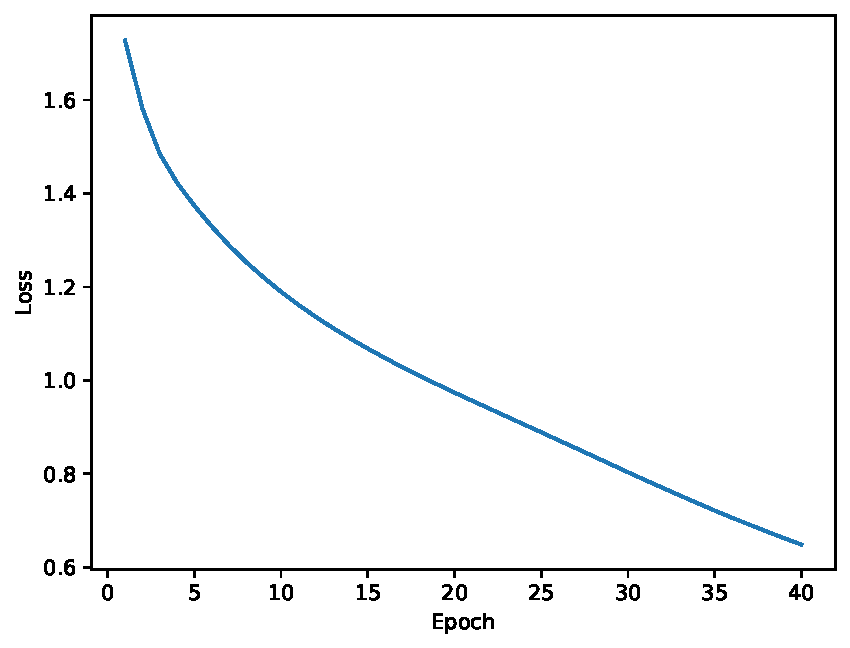
\includegraphics[width=\imagewidth]{q2/q2_1_lr-0.01-train-loss.pdf}
        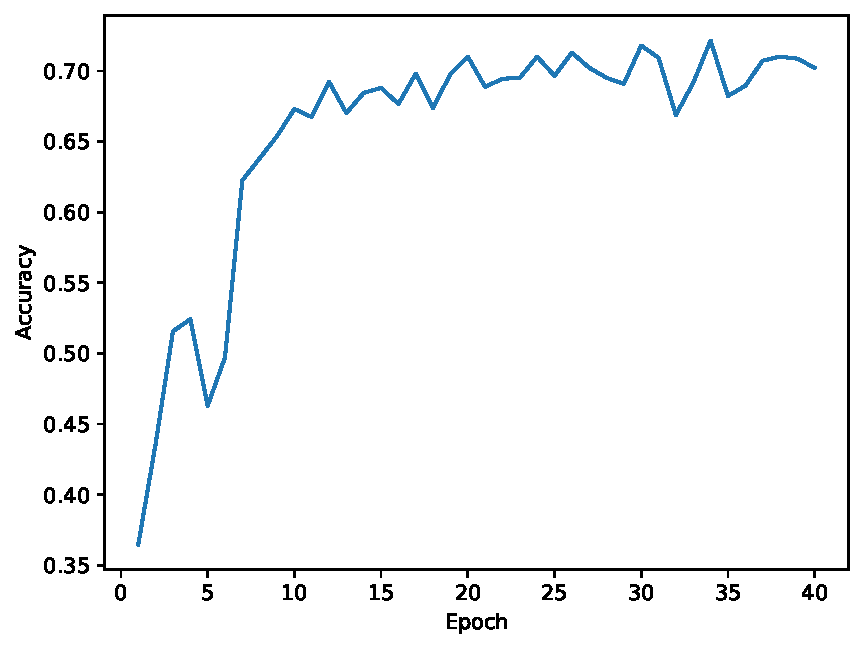
\includegraphics[width=\imagewidth]{q2/q2_1_lr-0.01-valid-accuracy.pdf} \\
        Final validation accuracy: 0.7023 \\
        Final test accuracy: 0.6927

    \subsection{2.}
        Plots of the training loss (left) and the validation accuracy (right) as a function of the epoch number: \\
        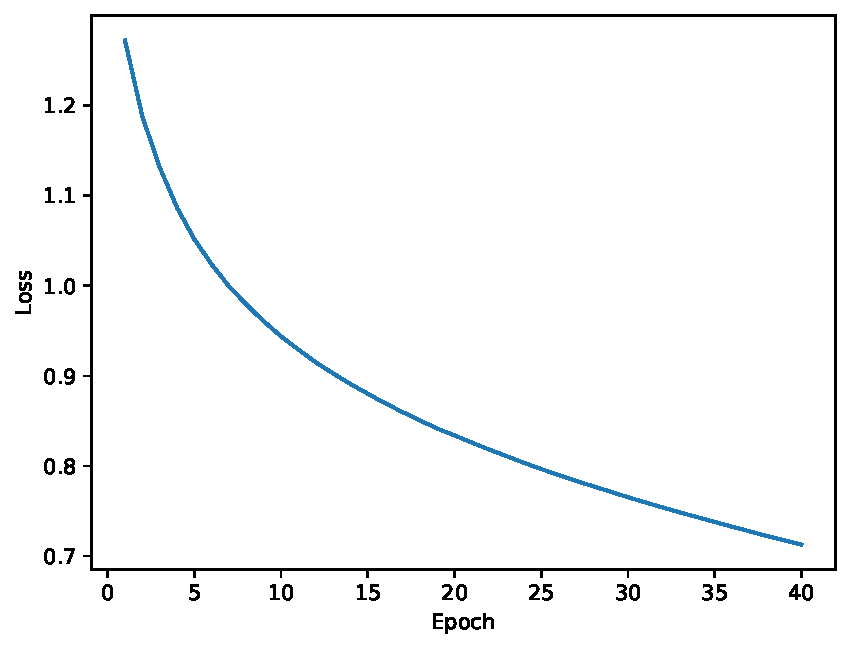
\includegraphics[width=\imagewidth]{q2/q2_2_lr-0.01-train-loss.pdf}
        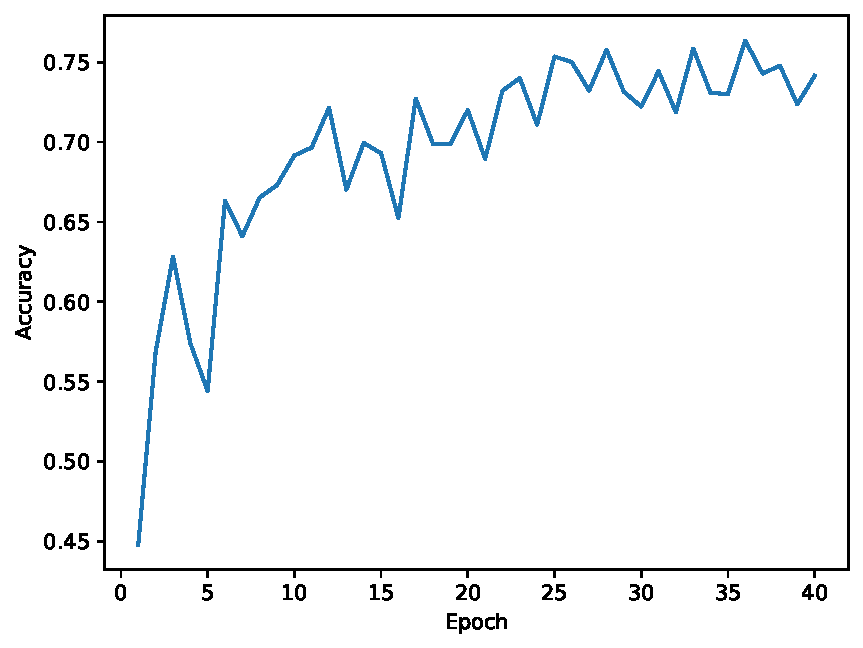
\includegraphics[width=\imagewidth]{q2/q2_2_lr-0.01-valid-accuracy.pdf} \\
        Final validation accuracy: 0.7415 \\
        Final test accuracy: 0.7280

    \newpage
    \subsection{3.}
        In the model of Question 2.1., without batch normalization, the number of trainable parameters is 5340742, whereas in the model of Question 2.2., with batch normalization and global average pooling, the number of trainable parameters is 755718. \\
        The number of trainable parameters includes the weights and biases of the convolutional and fully connected layers. In Question 2.2., additional trainable parameters are introduced due to the inclusion of batch normalization layers. However, the global average pooling operation reduces the input dimensionality for the first fully connected layer, leading to fewer parameters in that layer. \\
        In terms of performance, the batch normalization in Question 2.2. improves convergence speed and generalization by normalizing activations within mini-batches. In Question 2.1., flattening results in a higher-dimensional input to the MLP, whereas the global average pooling in Question 2.2. reduces the number of trainable parameters in the MLP block, mitigating overfitting and enhancing translation invariance. These factors contribute to the superior performance of the model in Question 2.2.

    \subsection{4.}
        In convolutional neural networks, small kernels are preferred over large ones because they reduce the number of trainable parameters and computational cost while allowing the stacking of multiple layers to achieve a larger receptive field with added non-linearities. This enhances feature extraction and improves parameter efficiency. Pooling layers, on the other hand, reduce spatial dimensions, lowering memory and computational requirements. They also introduce translation invariance, making the network robust to input variations, and help prevent overfitting by reducing the total parameter count. Together, small kernels and pooling layers enable efficient learning of hierarchical features while maintaining computational and parameter efficiency.


    \newpage
    \section{Question 3}
    \subsection{1. a)}
        Validation CER at the end of each epoch: \\
        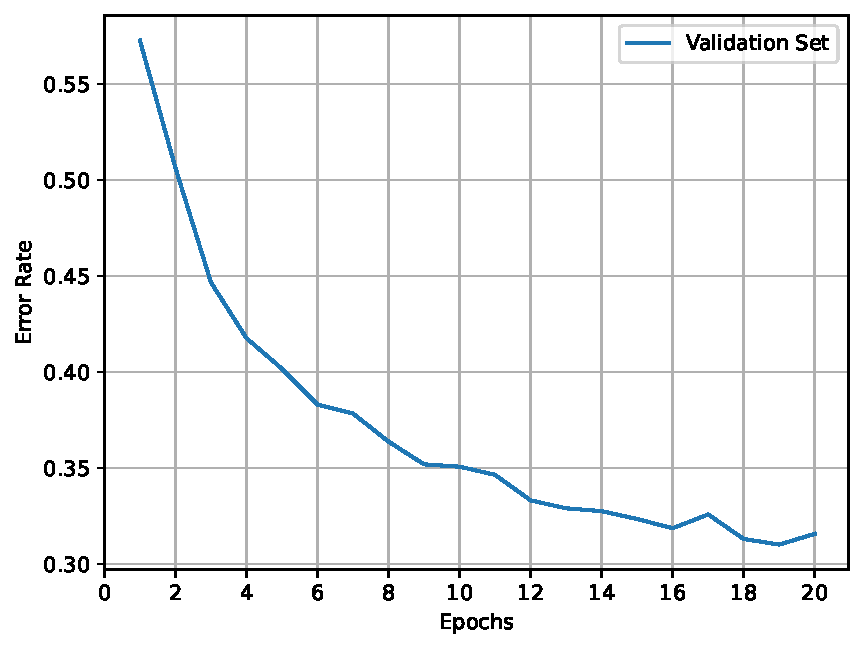
\includegraphics[width=\imagewidth]{q3/q3_1_no-attn.pdf} \\
        Test CER: 0.2989 \\
        Test WER: 0.7960

    \subsection{1. b)}
        Validation CER at the end of each epoch: \\
        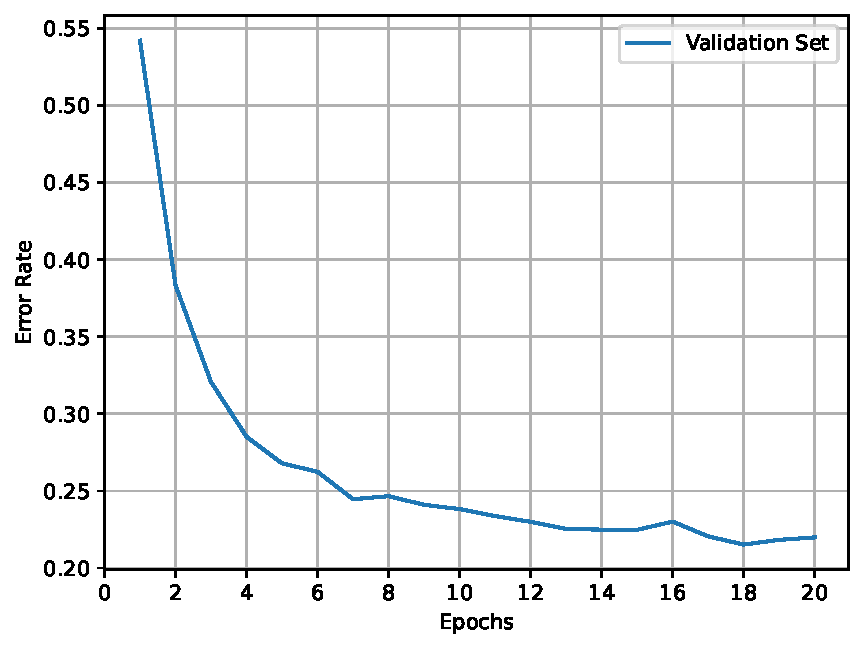
\includegraphics[width=\imagewidth]{q3/q3_2_attn.pdf} \\
        Test CER: 0.2127 \\
        Test WER: 0.7350        

    \subsection{1. c)}
        Test CER: 0.2166 \\
        Test WER: 0.7490 \\
        Test WER@3: 0.7100
        

\end{document}